In this section, the information that would facilitate the interpretation of the charts and reports produced by CodeMR is shared.

The CodeMR tool uses different visualization methods in the reports generated by the application of metrics. The charts are created with the help of these different visualization techniques based on the metric values obtained from the analysis conducted by the tool. Within this study's scope, the visualization methods known as "Metric Distribution" and "Package Structure" in CodeMR literature were preferred to present the results of the evaluations. The main reason for choosing this methods is that it makes the visual understanding of the results easier than other methods and also these methods provide a better situational perceptibility for projects. These visualization techniques were used to visualize the data obtained as a result of applying the metrics specified in section 3.2 and the analysis presented by CodeMR on complexity, coupling and cohesion concepts. Other visualization methods and charts are very detailed, and sharing such detailed results is beyond this study's scope. The tool also presents the values for each metric over the provided codebase and presents these values. Values for each metric are presented at project, module, package and class scopes. However, in the evaluations within the scope of this study, only the results of the metrics previously determined and explained in section \ref{section:3.2} were used. Fig \ref{fig:code-mr-metric-val} presents the metric values calculated with the help of the CodeMR Intellij IDEA plugin.
\begin{figure}[ht!]
    \centering
    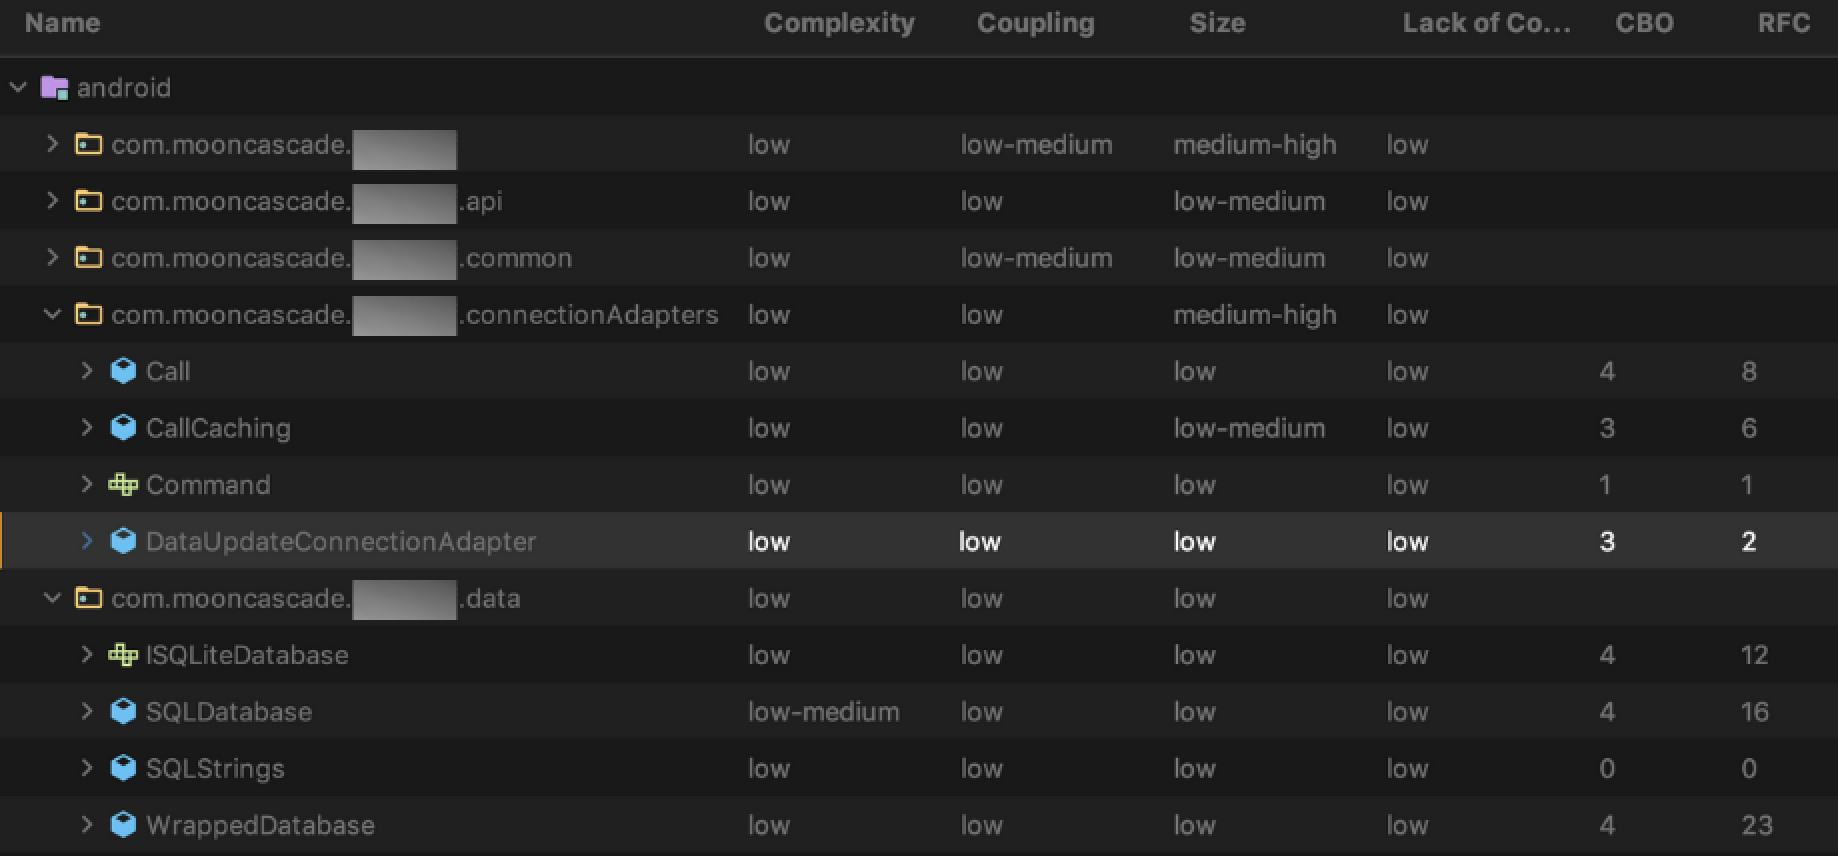
\includegraphics[scale=0.35]{figures/code-mr-metric-val.png}
    \caption{CodeMR Metric Value Presentation}
    \label{fig:code-mr-metric-val}
\end{figure}
\FloatBarrier

There are two important points to be aware of when interpreting the charts created by these methods using CodeMR. The first of these points is legends used to indicate metric levels. As can be seen in Fig. \ref{fig:code-mr-legends}, each colour corresponds to a metric level that is represented by a certain metric value threshold. 
\begin{figure}[ht!]
    \centering
    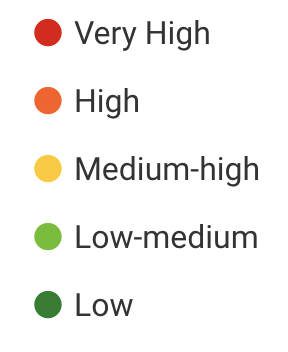
\includegraphics[scale=0.7]{figures/code-mr-legends.png}
    \caption{CodeMR Metric Level Indicators}
    \label{fig:code-mr-legends}
\end{figure}
\FloatBarrier

The second important point is how the percentages on these charts are calculated while realizing the charts created by CodeMR. There might be different metric levels in different percentages in the charts. These percentages of metric levels for the selected metrics are illustrated in charts proportionally to the code size of classes in this level. Detailed information about the formulas used in calculating metric values and how the values are interpreted amd visualized can be accessed through the CodeMR documentation\footnote{\label{fn:codemr} \url{https://www.codemr.co.uk/documents/}}.

Presentation of the results obtained via CoreMR is done as explained below. The charts and the  metrics values obtained from the evaluation have been shared for the project level. Although these techniques can be applied at the class and package level, it was preferred to present the project level results. It would not be very effective and useful to present these results for each class and package since there are many classes and packages for both codebases. On the other hand, at the class level, for making some evaluation and comparison, a few sample classes with high functionality were selected from both codebases, and they were evaluated and compared. Also, in accordance with the confidentiality requirements, the package and class names that will call the application name were hidden in the shared analysis results and figures. Then the results were presented via visualisation methods and numeric values. In the following sections, the results of this evaluation and the findings for comparisons are shared.

%$^{\ref{fn:codemr}}$.

